\chapter{Phương pháp đề xuất}
\label{chapter:proposed}
\ifpdf
    \graphicspath{{Chapter3/Chapter3Figs/PNG/}{Chapter3/Chapter3Figs/PDF/}{Chapter3/Chapter3Figs/}}
\else
    \graphicspath{{Chapter3/Chapter3Figs/EPS/}{Chapter3/Chapter3Figs/}}
\fi

\markboth{\MakeUppercase{\thechapter. Tích hợp thông tin không gian ảnh vào chỉ mục ngược}}{\thechapter. Tích hợp thông tin không gian ảnh vào chỉ mục ngược}

Rất nhiều công trình được đưa ra để giải quyết bài toán truy vấn ảnh như đã trình bày trong Mục \ref{local-features} và \ref{bag-of-words}). Tuy nhiên các phương pháp trên còn tồn tại những hạn chế mà một trong số đó là việc bỏ qua thông tin không gian ảnh. Trong khi đó cũng có nhiều phương pháp được đưa ra trong những năm gần đây để giải quyết vấn đề này được giới thiệu trong mục \ref{spatial}, nhưng cũng chưa thực sự hiệu quả. Điển hình là phương pháp spatial pyramid matching\cite{lazebnik2006beyond} sử dụng thông tin không gian ảnh để cải thiện độ chính xác nhưng chi phí tính toán lại rất lớn, thời gian phản hồi chậm nên khó có thể đáp ứng những bộ dữ liệu ngày càng lớn như hiện nay.

Trong chương này, chúng tôi sẽ trình bày phương pháp đề xuất tích hợp thông tin không gian ảnh vào chỉ mục ngược, với mục tiêu cân bằng độ chính xác truy vấn và thời gian phản hồi. Trước tiên chúng tôi nhắc lại những công trình khơi nguồn ý tưởng cho phương pháp đề xuất, sau đó trình bày chi tiết về ý tưởng cải tiến và phương pháp đề xuất.

\section{Chỉ mục ngược được sử dụng hiệu quả trong mô hình Bag-of-words}
\label{sec:inverted-index}
Như đã được giới thiệu sơ lược trọng mục \ref{matching}, chỉ mục ngược (inverted index) là phương pháp phổ dùng để tăng tốc độ truy vấn cơ sở dữ liệu bằng việc lưu trữ trước một ánh xạ từ nội dung đến vị trí trong cơ sở dữ liêu. Nói cách khác, chỉ mục ngược là một cấu trúc dữ liệu chủ yếu bao gồm 2 trường là khóa và giá trị. Mỗi khóa đại diện cho một \textit{từ}, và phần giá trị của tương ứng lưu trữ danh sách các văn bản có chứa từ đó. Vì vậy ta có thể dễ dàng lấy được danh sách tất cả các văn bản chứa từ truy vấn.

Chính vì sự thành công của các kỹ thuật tìm kiếm văn bản, chỉ mục ngược đã được mở rộng để sử dụng cho tìm kiếm ảnh trên cơ sở dữ liệu lớn. Để có thể xây dựng chỉ mục ngược cho cơ sở dữ liệu ảnh, mô hình BoW đã được sử dụng để biểu diễn hình ảnh. Quá trình xây dựng chỉ mục ngược như sau: (i) một bộ dò tìm các đặc trưng sẽ phát hiện những điểm quan trọng trên từng hình ảnh trong bộ dữ liệu, sau đó một bộ mô tả sẽ trích rút trích được những đặc trưng xung quanh điểm đó; (ii) các đặc trưng được gom thành các cụm để tạo thành từ điển, mỗi cụm là một tập các đặc trưng gần giống nhau và trung tâm của mỗi cụm là một visual word, mỗi visual word sẽ được gán một mã số khác nhau; (iii) Trường giá trị trong tệp chỉ mục ngược sẽ lưu trữ danh sách các hình ảnh có chứa các visual word tương ứng. Quá trình tạo tập chỉ mục ngược (inverted file) được minh họa trong Hình \ref{FigInvertedFile}.

\begin{figure}[!htbp]
  \begin{center}
    \leavevmode
    \ifpdf
      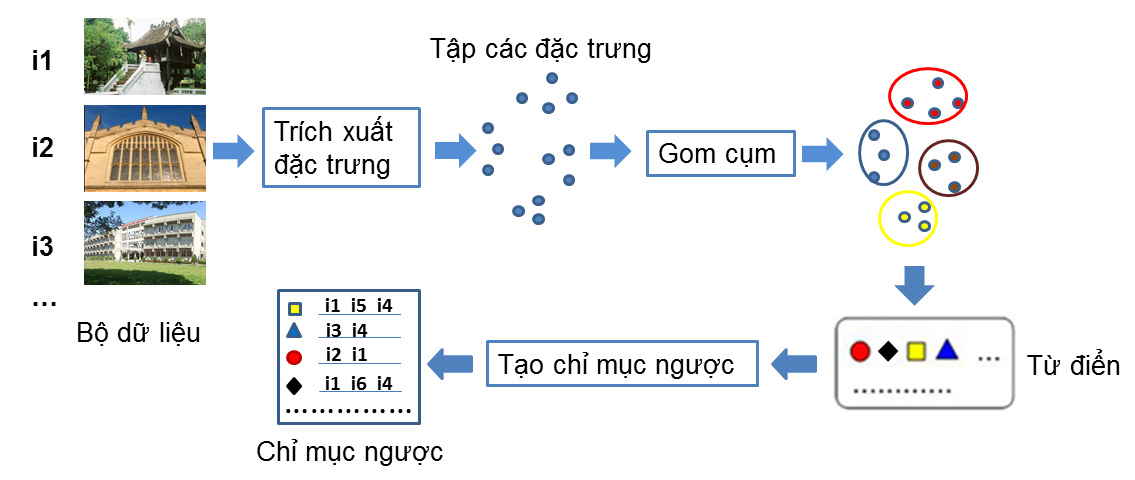
\includegraphics[scale=0.51]{invertedFile}
    \else
      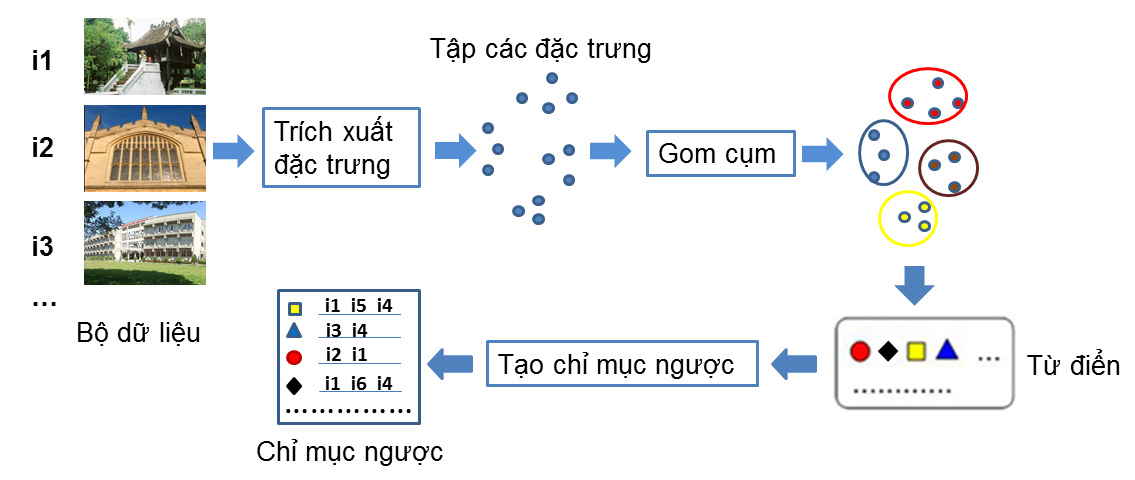
\includegraphics[scale=0.51]{invertedFile}
    \fi
    \caption[Quá trình tạo chỉ mục ngược]{Quá trình tạo chỉ mục ngược.}
    \label{FigInvertedFile}
  \end{center}
\end{figure}

Với cấu trúc hết sức đơn giản nhưng chỉ mục người lại cho thấy hiệu quả to lớn của nó. Chẳng hạn khi có một hình ảnh truy vấn được đưa vào, có thể dễ dàng tìm tất cả các hình ảnh liên quan tới nó mà không cần quan tâm tới những hình ảnh không liên quan khác, hoặc trong quá tính trọng số tf-idf cho một visual word được trình bày trong mục \ref{matching} cũng có thể nhanh chóng tìm tất cả những hình ảnh chứa visual words đó mà không phải truy xuất vào dữ liệu của từng hình ảnh.

Với việc sử dụng chỉ mục ngược, tốc độ truy vấn được tăng lên đáng kể. Cũng chính vì vậy, chúng tôi đề xuất ý tưởng tích hợp thông tin không gian ảnh vào chỉ mục ngược nhằm tận dụng tính đơn giản nhưng hiệu quả của nó.

\section{Tích hợp thông tin không gian ảnh vào chỉ mục ngược}
\label{sec:intergrated}
Phương pháp chúng tôi đề xuất bắt nguồn từ ý tưởng tận dụng tính hiệu quả của chỉ mục ngược và việc sử dụng thông tin không gian ảnh trong công trình nghiên cứu của Lazebnik và các đồng nghiệp\cite{lazebnik2006beyond}. Để tận dụng thông tin không gian ảnh của mỗi visual word, chúng tôi chia các hình ảnh thành nhiều ô tại nhiều cấp độ khác nhau. Với mỗi ô tại mỗi cấp độ, chúng tôi lọc được các visual word của tất cả các hình ảnh có chứa visual này trong ô đang xét. Từ đó xây dựng được một chỉ mục ngược cho mỗi ô tại mỗi cấp độ. Mỗi chỉ mục ngược thể hiện một ô trong không gian ảnh, sẽ lưu trữ tất cả các visual word của bộ dữ liệu có nằm trong ô mà nó thể hiện, đồng thời lưu trữ chỉ số của các hình ảnh mà visual word này có nằm trong ô đó của các hình ảnh đó. Chẳng hạn, khi sử dụng hai cấp độ, ở cấp độ thứ nhất hình ảnh không bị chia, tức là mỗi một hình ảnh chỉ có một ô thể hiện cả hình ảnh đó, chỉ mục ngược cho ô này chính là chỉ mục ngược cơ bản. Tại cấp độ thứ hai, hình ảnh được chia làm bốn phần, mỗi ô là một góc phần tư. Với mỗi góc phần tư trong mỗi hình ảnh sẽ tìm được các visual word nằm trong góc này, và khi duyệt qua toàn bộ bộ dữ liệu ta sẽ xây dựng được một chỉ mục ngược cho góc phần tư này. Tại quá trình truy vấn, khi một hình ảnh được đưa vào, nó sẽ được chia ra như trong quá trình tạo chỉ mục ngược đã thực hiện trước đó. Với mỗi ô tại mỗi cấp độ, các visual word sẽ được lọc ra trong hình ảnh truy vấn này, từ đó đưa vào chỉ mục ngược tương ứng với ô đó để tìm ra tất cả những hình ảnh cũng chứa visual word này tại ô này. 

Cụ thể hơn, theo nghiên cứu của Lazebnik, hình ảnh được chia thành nhiều phần sử dụng lưới ô vuông phân cấp (hay còn được gọi là không gian phân cấp - spatial pyramid). Một lưới ô vuông tại cấp \textit{l} sẽ chia hình ảnh thành $2^l \times 2^l$ ô với kích cỡ như nhau. Do đó, số ô vuông trên lưới ở cấp 0 là $1 \times 1$; cấp 1 là $2 \times 2$. Nếu cấp \textit{l} càng cao thì lưới ô vuông sẽ càng dày đặc hơn. Nếu coi mỗi ô của hình ảnh được chia bởi lưới ô vuông phân cấp là một hình ảnh độc lập, dựa trên mô hình BoW ta sẽ tính được các biểu đồ độc lập. Chính vì mức độ chia tiết của các biểu đồ khác nhau nên chúng sẽ được đánh trọng số khác nhau rồi rồi được ghép nối với nhau để tạo thành một véc tơ đặc trưng biểu diễn cho hình ảnh, độ dài của véc tơ này sẽ tăng $\frac{1}{3}\times(4^{L+1} - 1)$ lần. Bằng cách biểu diễn như vậy, các hình ảnh có sự phân bố các visual word tương tự nhau sẽ được biễu diễn bằng những biểu đồ ghép nối gần giống nhau.

Trong phương pháp đề xuất này, chúng tôi chỉ áp dụng cách chia hình thành không gian phân cấp theo nghiên cứu trên, sau đó kết quả của quá trình chia hình được sử dụng một cách hoàn toàn khác. Phương pháp của Lazebnik cho thấy độ thức tạp lớn trong quá trình so khớp, vì vậy nó thường sử dụng để hậu xử lý kết quả. Còn trong phương pháp của chúng tôi, thông tin không gian ảnh được tích hợp vào chỉ mục ngược, được sử dụng ngay trong bước tiền xử lý, không làm tăng thêm nhiều chi phí tính toán.

Để sử dụng thông tin không gian ảnh đã được tích hợp vào chỉ mục ngược, chúng tôi đề xuất xử dụng một kỹ thuật xếp hạng được gọi là \textit{bầu chọn} (voting). Kỹ thuật được định nghĩa như sau: 

Trong quá trình truy vấn, các đặc trưng sẽ được rút trích từ hình ảnh truy vấn, sau đó từ các đặc trưng ta sẽ lấy được các visual word bằng cách sử dụng từ điển sau đó tra cứu trong tập chỉ mục ngược để lấy được các hình ảnh ứng viên. Những hình ảnh nào có số lượng visual word trùng với các visual word trong hình ảnh truy vấn càng nhiều thì sẽ càng được xếp hạng cao hơn trong danh sách kết quả truy vấn trả về.

Với kỹ thuật bầu chọn trong phương pháp đề xuất, chúng tôi duyệt qua tất cả các ô ở tất cả các cấp khác nhau để thực hiện việc bầu chọn. Do đó, nếu hai hình ảnh chứa các visual word giống nhau trong cùng một ô sẽ nhận được nhiều lượt bầu chọn hơn so với hai hình ảnh có các visual word giống nhau nhưng lại nằm rải rác ở các ô khác nhau. Các lượt bầu chọn sẽ được đánh trọng số tùy theo từng cấp để thể hiện mức độ quan trọng của các cấp độ chia hình ảnh khác nhau. Chúng tôi đánh trọng số giống phương pháp của Lazebnik\cite{lazebnik2006beyond}. Trọng số tại cấp \textit{l} sẽ là $\frac{1}{2^{L}} + \sum\limits{l=1}^L \frac{1}{2^{L-l+1}}$. Đây là phương pháp đánh trọng số được đề xuất bởi K. Grauman and T. Darrell\cite{grauman2005pyramid}.

Một trong những điểm đặc biệt của phương pháp đề xuất là chúng tôi sử dụng đa chỉ mục ngược. Tức là chia thành nhiều tập chỉ mục ngược khác nhau nhưng các tập vẫn giữ được cấu trúc căn bản của chỉ mục ngược. Mỗi tập sẽ dùng để lưu trữ chỉ muc cho một ô trên không gian phân cấp. Nếu cấp độ cao nhất của không gian phân cấp là \textit{L} thì tổng số lượng tập chỉ mục ngược sẽ là $\frac{1}{3}(4^{L+1} - 1)$ và mỗi cấp độ sẽ có $2^l \times 2^l$ tập chỉ mục ngược với $0 \leq l \leq L$. Hình \ref{FigBasicIdea} mô tả khái quát cho phương pháp được đề xuất.

\begin{figure}[!htbp]
  \begin{center}
    \leavevmode
    \ifpdf
      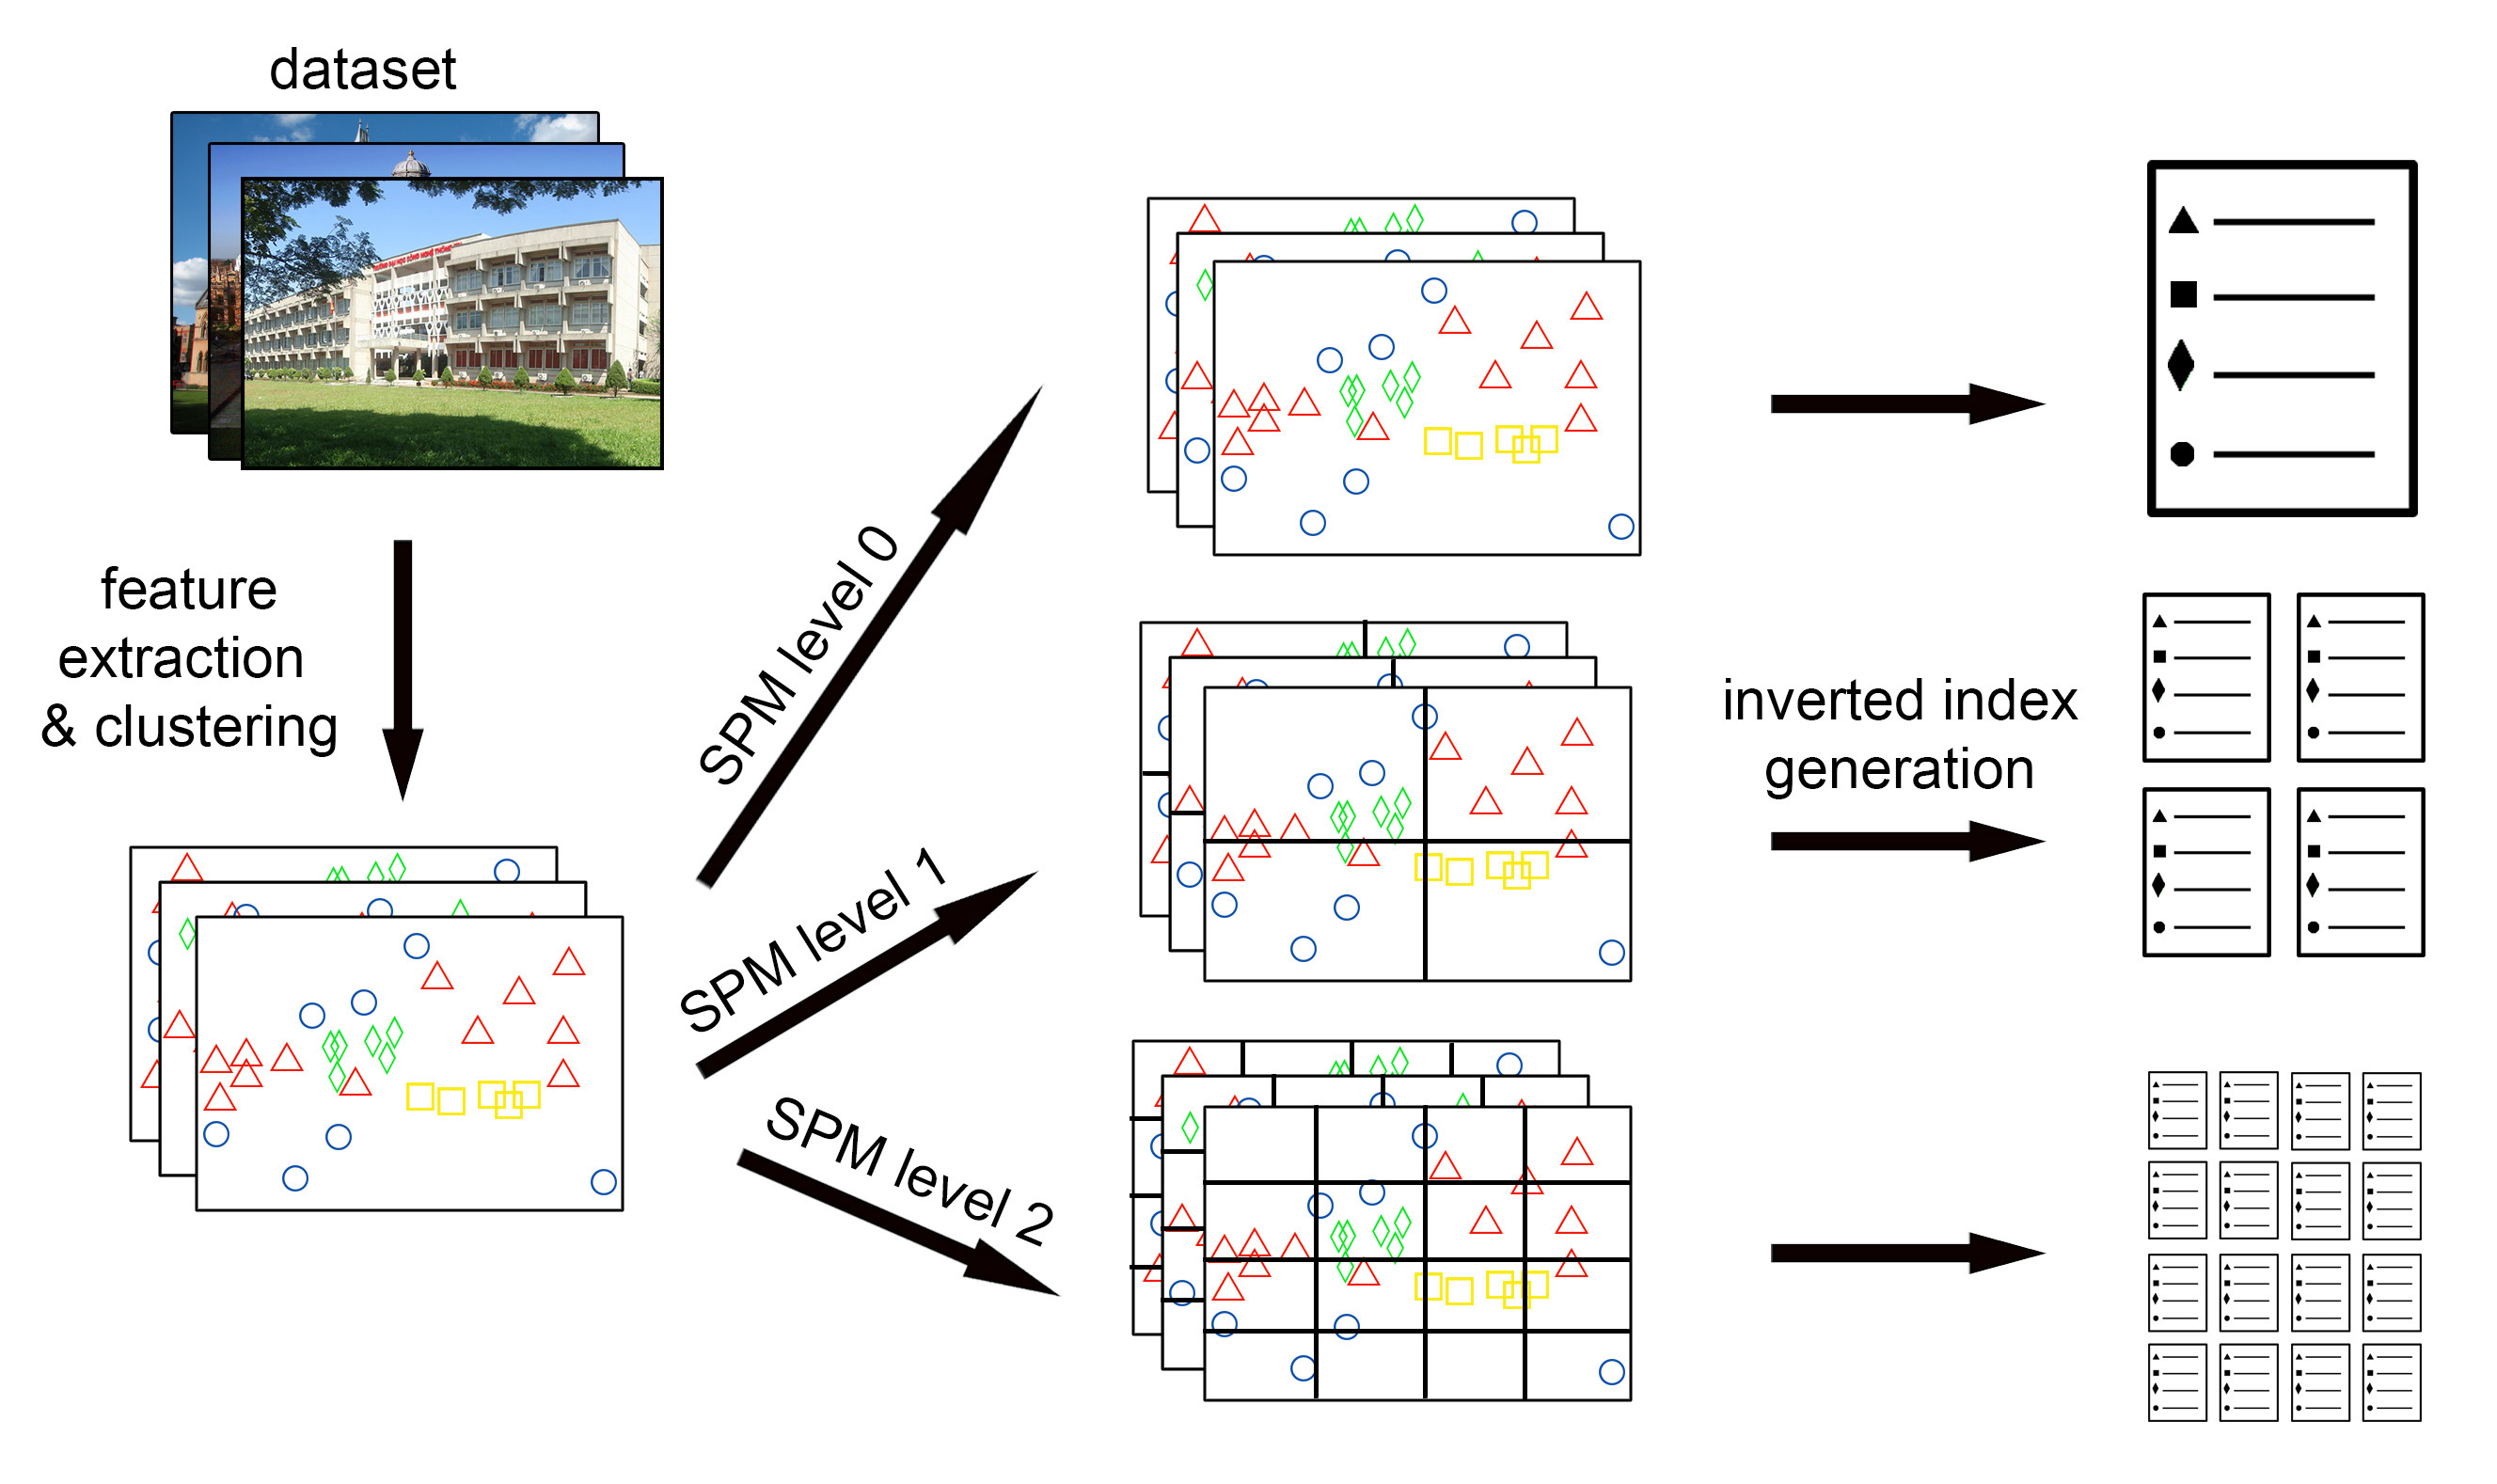
\includegraphics[scale=0.15]{basicIdea}
    \else
      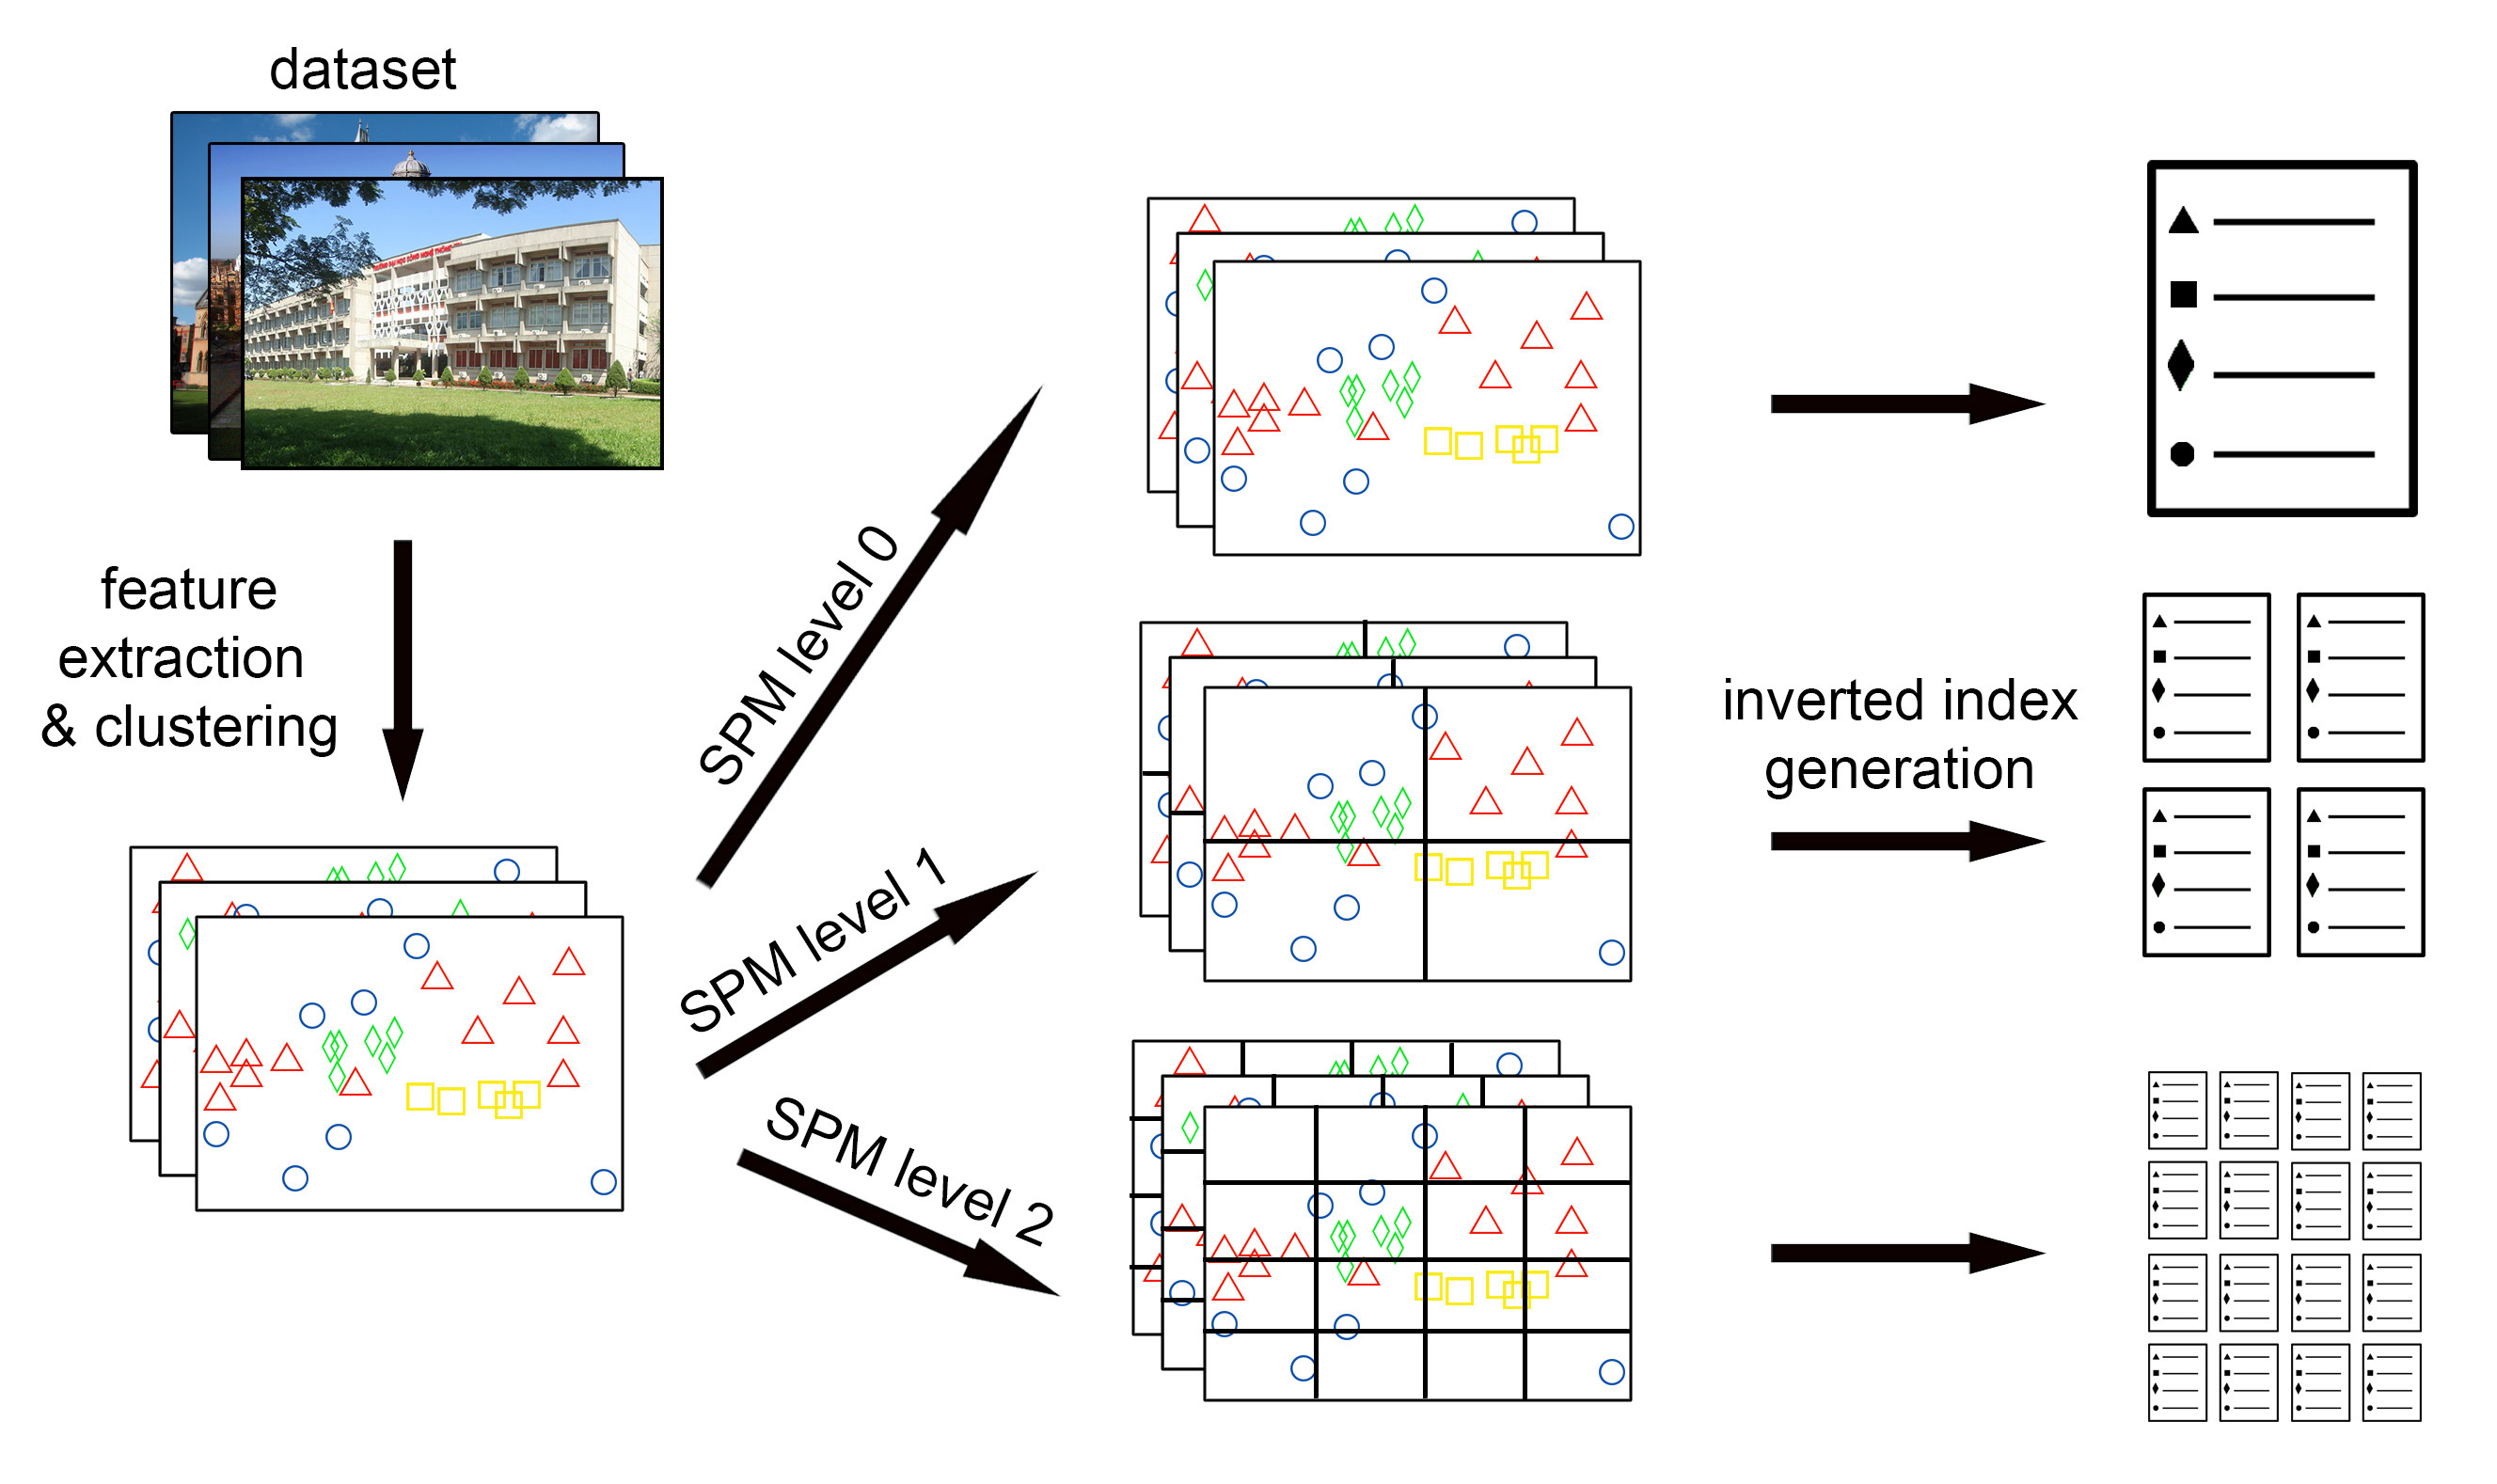
\includegraphics[scale=0.15]{basicIdea}
    \fi
    \caption[Khái quát về phương pháp đề xuất]{Khái quát về phương pháp đề xuất.}
    \label{FigBasicIdea}
  \end{center}
\end{figure}

Khi thực hiện quá trình rút trích các đặc trưng cho tất cả các hình trong cơ sở dữ liệu, thông tin không gian của các đặc trưng đó sẽ được lưu trữ lại. Sau đó các bộ mô tả (descriptors) của đặc trưng (ví dụ như key points) sẽ được lượng tử hóa để tạo thành một bảng từ vựng của các visual word (từ điển). Mỗi hình ảnh sẽ chứa một tập các visual word. Tiếp đó ta sẽ sử dụng không gian phân cấp để chia tất cả các hình ảnh thành các ô nhỏ với "độ mịn" tăng dần dựa trên cấp được định nghĩa. Lúc này, thông tin không gian của các đặc trưng đã được lưu trước đó sẽ được sử dụng để xác định xem visual word đó có thuộc ô đang xét hay không. Tất cả các visual word được tìm thấy trong mỗi ô sẽ được thu thập lại. Tiếp theo, tập hợp của các visual word được tìm thấy trong mỗi ô của các hình ảnh sẽ được dùng để sinh ra một tập chỉ mục ngược tương ứng với ô đó. Số lượng tập chỉ mục ngược được sinh ra bằng với tổng số ô của không gian phân cấp.

Trong quá trình truy vấn, các đặc trưng cũng được rút trích từ hình ảnh truy vấn. Sau đó chúng được đưa vào từ điển để lấy được các visual word tương ứng. Dựa vào vị trí của các visual word này, ta có thể xác định được chúng thuộc ô nào tại mỗi cấp của mô hình không gian phân cấp. Từ đó ta có thể có thể truy xuất ngay lập tức tới tập chỉ mục ngược tương ứng với mỗi ô để lấy và xếp hạng danh sách hình ảnh ứng viên một cách đồng thời. Ta xếp hạng hình ảnh bằng phương pháp bầu chọn nên việc bầu chọn diễn ra trong mỗi lần truy xuất tập chỉ mục ngược, do đó danh sách đếm số lượt bầu chọn sẽ được cập nhật liên tục trong suốt quá trình truy xuất các tập chỉ mục ngược. Khi quá trình bầu chọn kết thúc, ta sẽ tổng hợp toàn bộ số lượt bầu chọn cho từng hình rồi xếp hạng các hình theo số lượt bầu chọn. Toàn bộ quá trình truy vấn của phương pháp đề xuất được minh họa trong Hình \ref{FigQueryProcess}.

\begin{figure}[!htbp]
  \begin{center}
    \leavevmode
    \ifpdf
      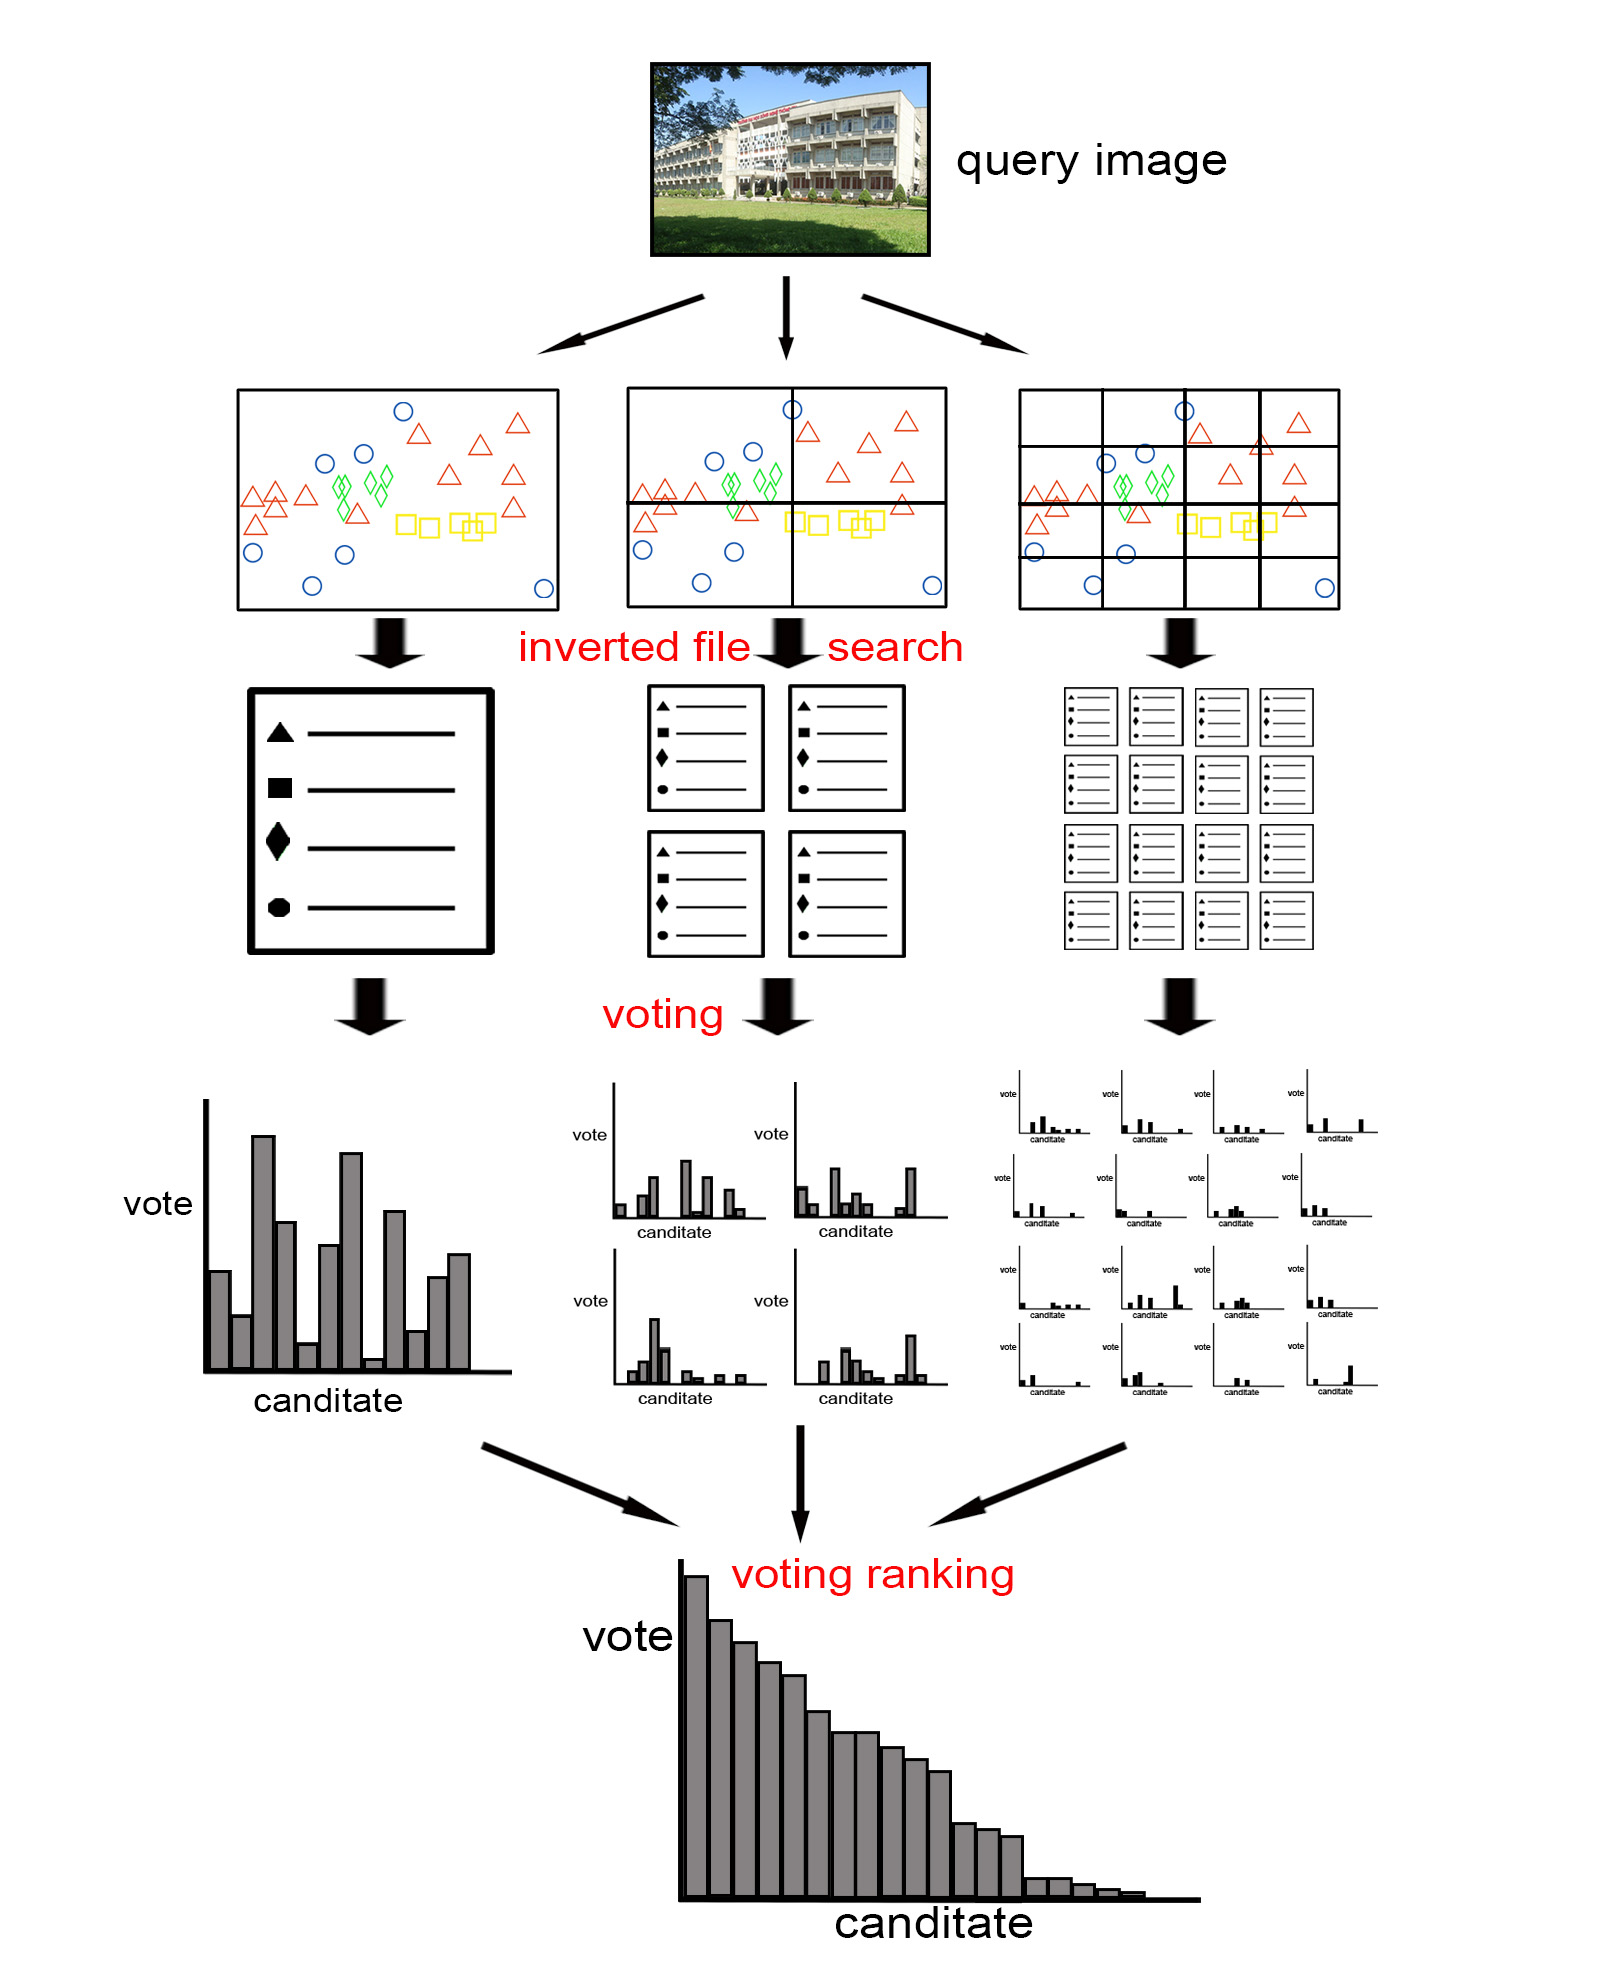
\includegraphics[scale=0.25]{queryProcess}
    \else
      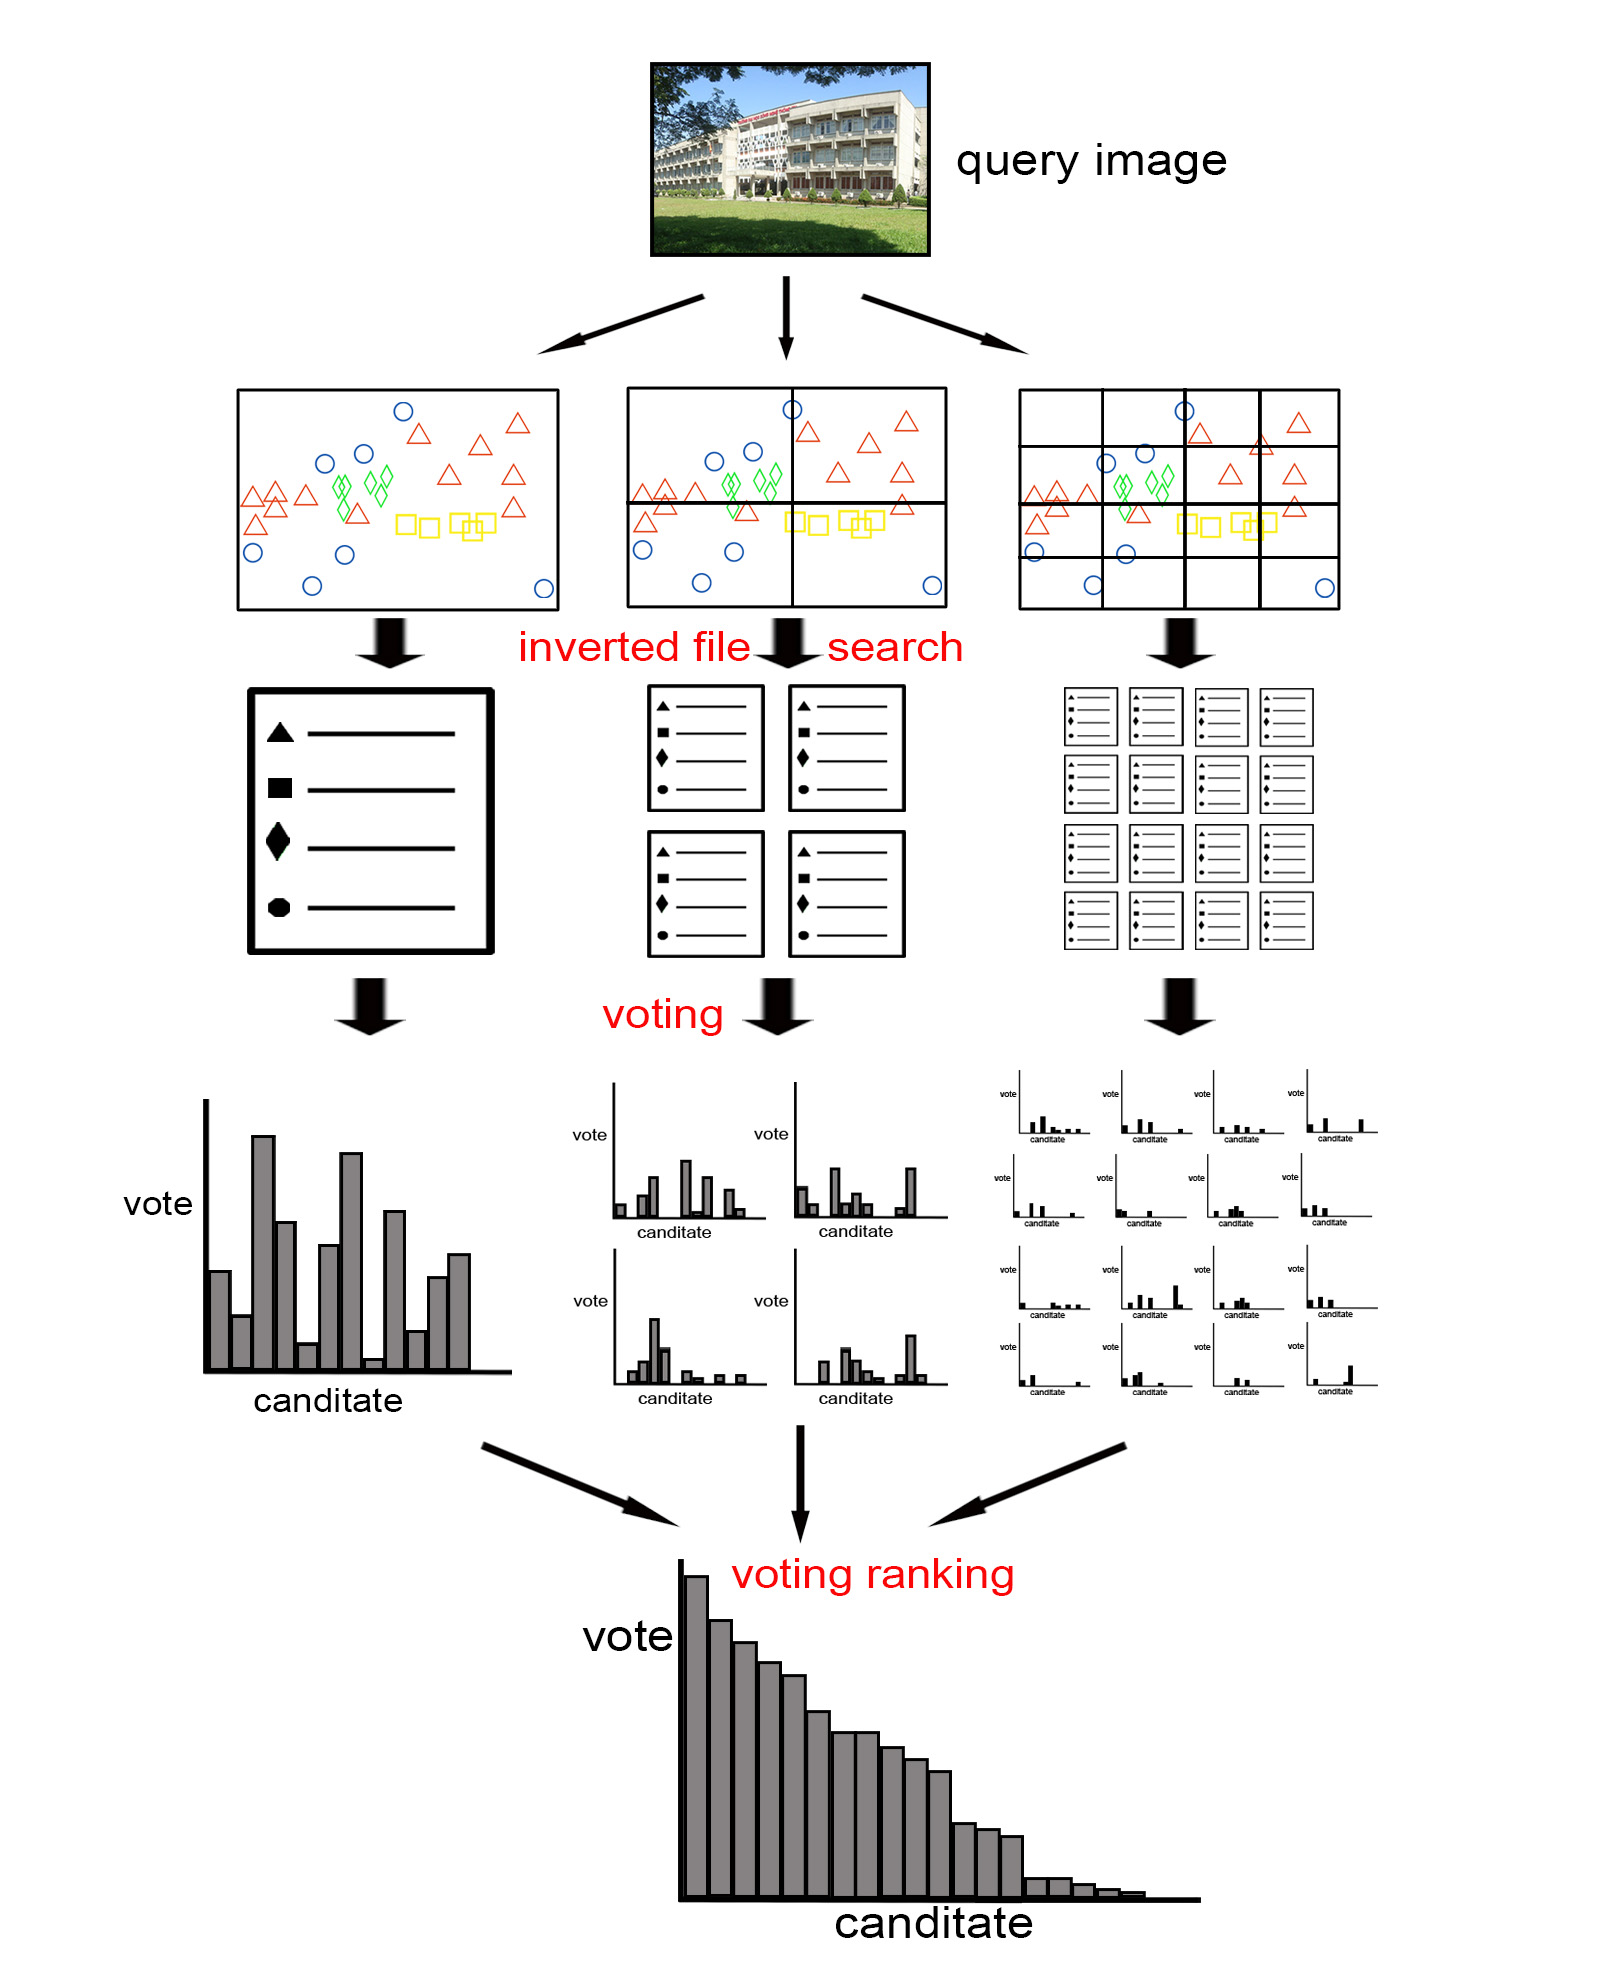
\includegraphics[scale=0.25]{queryProcess}
    \fi
    \caption[Quá trình truy vấn của phương pháp đề xuất]{Quá trình truy vấn của phương pháp đề xuất.}
    \label{FigQueryProcess}
  \end{center}
\end{figure}